\documentclass{article}

%-------------------------%
% PREAMBUŁA --------------%
%-------------------------%
\usepackage[utf8]{inputenc}
\usepackage[OT4]{polski}
\usepackage{caption}
\usepackage{amsmath}
\usepackage{tikz}
\usepackage{subcaption}
\usepackage{tabularx}
%\usepackage{wrapfig}
\usepackage{caption}
\usepackage{array}
\usepackage{hyperref}
\usepackage{graphicx}
%\usepackage{color}
%\usepackage{epstopdf}
\usepackage{fancyhdr}
\usepackage[justification=centering]{caption}
\usepackage[margin=60pt]{geometry}



%------- Typy kolumn do ustawiania szerokości ------- %
\newcolumntype{L}[1]{>{\raggedright\let\newline\\\arraybackslash\hspace{0pt}}m{#1}}
\newcolumntype{C}[1]{>{\centering\let\newline\\\arraybackslash\hspace{0pt}}m{#1}}
\newcolumntype{R}[1]{>{\raggedleft\let\newline\\\arraybackslash\hspace{0pt}}m{#1}}

\renewcommand{\arraystretch}{1.3}







\begin{document}

%-------------------------%
%Tabela nagłówkowa -------%
%-------------------------%

\begin{table}[h]
\begin{tabular}{|l|l|l|l|l|l|}
\hline
\begin{tabular}[c]{@{}l@{}}
Wydział:\\ WFiIS\end{tabular} &
\multicolumn{2}{l|}{\begin{tabular}[c]{@{}l@{}}
Imię i nazwisko:\\ 1. Axel Zuziak\\ 2. Marcin Węglarz \end{tabular}} 
& Rok \textbf{II}         
& Grupa \textbf{02}          
& Zespół \textbf{03}      \\ \hline
\textbf{\begin{tabular}[c]{@{}l@{}}
PRACOWNIA\\ FIZYCZNA \\ WFiIS AGH\end{tabular}} &
\multicolumn{4}{l|}{ Temat:\textbf{ Dyfrakcja światła.} }                                                                                                                       & \multicolumn{1}{c|}{\begin{tabular}[c]{@{}c@{}}
Nr ćwiczenia\\ \textbf{71}
\end{tabular}} \\ \hline
\begin{tabular}[c]{@{}c@{}}
Data wykonania:\\ 22.04.2015
\end{tabular} &
\begin{tabular}[c]{@{}c@{}}
 Data oddania:\\ 29.04.2015
\end{tabular} &
\begin{tabular}[c]{@{}c@{}}
Zwrot do poprawy: \\ 
\end{tabular}                                 
& 
\begin{tabular}[c]{@{}c@{}}
Data oddania: \\ 
\end{tabular}&
\begin{tabular}[c]{@{}c@{}}
Data zaliczenia:\\
\end{tabular}& 
\begin{tabular}[c]{@{}c@{}}
OCENA:\\
\end{tabular}       
\\ & & & & & \\ \hline
\end{tabular}
\end{table}
%-----Koniec tabeli------
\begin{abstract}
	W ćwiczeniu badano dyfrakcję monochromatycznego światła laserowego o długości fali 650 nm na szczelinach podwójnej oraz pojedynczej. Przy pomocy fotodiody jako detektora natężenia światła mierzono natężenie światła padającego na ekran. Poprzez wyznaczenie odległości pomiędzy kolejnymi maksimami natężenia oraz poprzez zmierzenie odległości szczelin od ekranu wyznaczono  szerokość szczelin oraz dla przypadku dwóch szczelin odległość między ich środkami. 
\end{abstract}

\section{Wstęp}
Zarówno zjawisko dyfrakcji jak i interferencji są przykładami na falowy charakter światła. O zjawisku interferencji mówimy w przypadku dwóch szczelin dla których ich szerokość $a<<\lambda$, gdzie $\lambda$ jest długością fali padającej. Jeżeli rozpatrzymy dowolny punkt $P$ na ekranie i będziemy chcieli policzyć dla niego wypadkową amplitudę fali padającej będziemy musieli dodać do siebie fale padające z różnych szczelin. Schematycznie problem ten pokazano na Rysunku \ref{schemat_interferencja}.

\begin{figure}[h!]
	\centering
	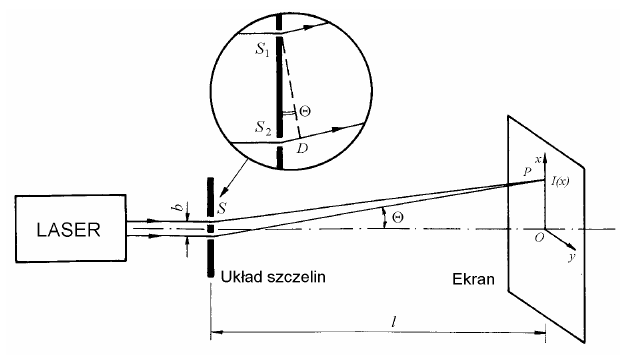
\includegraphics[width=0.7\textwidth]{images/interferencja.png}
	\caption{Schemat interferencji światła na dwóch szczelinach odległych od siebie o $b$.\cite{1}}
	\label{schemat_interferencja}
\end{figure}
Jak łatwo zauważyć na pomocniczym rysunku droga optyczna światła od szczeliny do punktu $P$ jest różna dla każdej ze szczelin. Konsekwencją tego faktu jest przesunięcie fazowe pomiędzy falami w punkcie $P$. \\
Przesunięcie fazowe, które oznaczmy przez $\varphi$, jest związane z kątem $\theta$ pod jakim obserwujemy punkt $P$ na ekranie, oraz odległością $b$ między szczelinami (Rysunek \ref{schemat_interferencja}) zależnością\cite{1}:
\begin{equation}
\varphi = \frac{2\pi}{\lambda}b \sin \theta
\label{wz_fi}
\end{equation}
Fala wypadkowa w punkcie $P$ wynosi:\\
$E=E_0\sin \omega t +E_0\sin (\omega t + \varphi)$\\\\
Korzystając z zależności trygonometrycznych można powyższe równanie przekształcić do postaci\cite{1}:\\\\
$E=[2E_0\cos (\varphi/2)]\sin(\omega t + \beta)$\\\\
Gdzie $\beta$ oraz $E_0$ są pewnymi stałymi. Natężenie światła jest proporcjonalne do kwadratu wypadkowej amplitudy drgań stąd:\\
$I\propto \cos ^2 \Big(\frac{\varphi}{2}\Big)$\\\\
Dodatkowo jeżeli odległość ekranu od szczelin jest duża w porównaniu do wymiarów obrazu na ekranie możemy przyjąć, że $\sin\theta \approx x/L$ ostatecznie wzór na natężenie przepiszemy w postaci:\\
\begin{equation}
I_{int}(x) = I_0\cos ^2 \Big(\frac{\pi bx}{L\lambda}\Big)
\label{wz_natezenie_interferencja}
\end{equation}
Z powyższego wzoru bezpośredio wynika, że maksima natężenie będą występowały dla punktów o współrzędnych:\\
$x_m = \frac{m\lambda L}{b}\ \ \ ,m=1,2,3,...$\\
oraz będą sobie równe (Rysunek \ref{rysunki_prazkow}a).\\

W rzeczywistym eksperymencie trudno jest uzyskać szerokość szczeliny o szerokości znacznie mniejszej od długości fali i obserwujemy zjawisko dyfrakcji. Chcąc rozpatrzyć dyfrakcję na pojedynczej szczelinie o szerokości $a$ musimy podzielić ją na $n$ odcinków i policzyć superpozycję drgań padających z każdego z tych odcinków (przy założeniu że długość odcinków dąży do zera). Dalsze wyprowadzenie można poprowadzić na przykład przedstawiając zaburzenia od poszczególnych fragmentów szczeliny w postaci wektorów przesuniętych w fazie o stały czynnik. Superpozycja takich zaburzeń jest więc sumą tych wektorów. Powyższe rozumowanie zostało przedstawione krok po kroku w podręczniku \cite{5}. Ostatecznie otrzymujemy (przy ponownym założeniu że odleglość od ekranu jest znacznie większa od rozmiarów obrazu)\cite{1}:
\begin{equation}
I_{dyf}(x) = I_0\Big(\frac{\sin \alpha}{\alpha}\Big)^2\text{  \hspace{0.1cm}  gdzie   \hspace{0.1cm}} \alpha=\frac{\pi a}{\lambda}\sin\theta \cong \frac{\pi a x}{\lambda L}
\label{wz_natezenie_dyfrakcyjne}
\end{equation}\\\\

W przypadku doświadczenia z jedną szczeliną będziemy wykorzystywać wzór (\ref{wz_natezenie_dyfrakcyjne}), dla doświadczenia z dwoma szczelinami końcowy efekt będzie złożeniem dwóch przedstawionych powyżej. Schemat natężenia światła na ekranie dla poszczególnych sytuacji przedstawia Rysunek \ref{rysunki_prazkow}. Ilościowo wartość natężenia dla interferencji fal światła na dwóch szczelinach o szerokości $a$ przedstawia wzór:
\begin{equation}
\begin{cases}
I(x) = I_0\Big(\frac{\sin \alpha}{\alpha}\Big)^2(\cos \beta)^2   \\
\beta \cong \frac{\pi b x}{\lambda L}\\
\alpha \cong \frac{\pi a x}{\lambda L}
\end{cases}
\end{equation}

dodaj prosze ten wzor dla jednej szczeliny:
\begin{equation}
	\label{pozycja_maks_jedna_szczelina_min}
	x_{min} = m\frac{\lambda L}{d}
\end{equation}
\begin{equation}
	\label{pozycja_maks_jedna_szczelina_max}
	x_{max} = (m+\frac{1}{2})\frac{\lambda L}{d}
\end{equation}


\section{Aparatura}
\begin{itemize}
	\item \textbf{Woltomierz cyfrowy} - \textit{"Digital voltometer type v560"}. Napięcie mierzono na zakresie $100$ mV. % dopisz proszę prawdziwe zakresy
	\item \textbf{Laser} o długości fali 650nm.
	\item \textbf{Linijka} o długości 150cm i najmniejszej podziałce = 0,1 cm.
	\item \textbf{Opornik regulowany dekadowy} 10x100$\Omega$ oraz dwa oporniki o oporze 1k$\Omega$ oraz 2k$\Omega$
	\item \textbf{Bateria zasilająca} 2 x 1.5V
	\item \textbf{Fotodioda} umieszczona w przesuwniku x-y (regulacja w pionie odbywałą się z dokładnościa 0.05 mm)
	\item \textbf{Płytki} z pojedynczymi oraz podwójnymi szczelinami
	
		
\end{itemize}
\begin{figure}[h!]
	\centering
	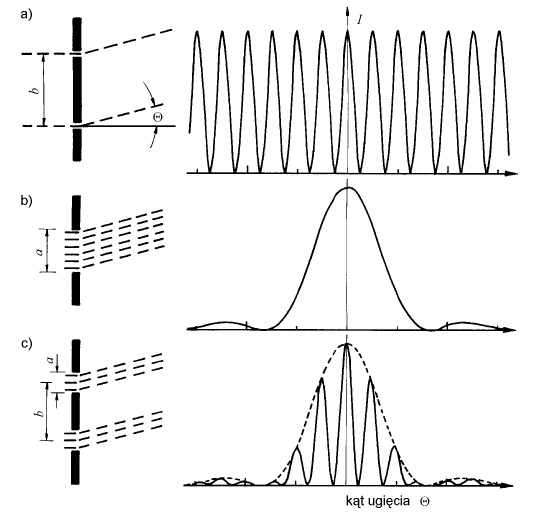
\includegraphics[width=0.7\textwidth]{images/prazki.png}
	\caption{Wykres natężenia światła na ekranie dla \textbf{a)} interferencji przy zachowaniu warunku $a<<\lambda$, \textbf{b)} dyfrakcji na pojedynczej szczelinie o szerokości $a$ oraz \textbf{c)} złożenie poprzednich zjawisk, interferencja fali padającej z dwóch szczelin o szerekości $a$ każda.\cite{1}}
	\label{rysunki_prazkow}
\end{figure}

\newpage
\section{Wyniki pomiarów}
\subsection{Pojedyncza szczelina}
Na wykresie \ref{jedna_szczelina_calosc} przedstawiono zależność natężenia światła od położenia detektora. Wykres jest zbiorem punktów pomiarowych połączonych krzywą gładką wygenerowaną przez program Gnuplot. W celu uwidocznienia położeń ekstremów narysowano wykres \ref{jedna_szczelina_log} z logarytmiczną skalą na osi Y. Odczytane maksima i minima przedstawiono w tabeli \ref{jedna_szczelina_tab_maks}. Korzystając ze wzorów \ref{pozycja_maks_jedna_szczelina_min} oraz \ref{pozycja_maks_jedna_szczelina_max} obliczono szerokość szczeliny $d$. Otrzymano cztery wyniki odpowiednio dla kolejnych maksimów i minimów. Oczywiście taka ilość wyników nie pozwala na posługiwanie się niepewnością typu $A$. Wyznaczono niepewność typu $B$ dla każdego wyniku korzystając z prawa przenoszenia niepewności.
\begin{equation*}
	u(d) = \sqrt{\left[\frac{m\lambda u(L)}{x} \right]^2 + \left[\frac{-m\lambda L u(x)}{x^2} \right]^2}
\end{equation*}
Powyższa niepewność jest tym większa im 
\begin{figure}[h!]
        \centering
        \begin{subfigure}[b]{\textwidth}
			\fontsize{6}{8}\selectfont % zmniejszam czcionke
			\centering
			\resizebox{0.9\textwidth}{!}{% GNUPLOT: LaTeX picture with Postscript
\begingroup
  \makeatletter
  \providecommand\color[2][]{%
    \GenericError{(gnuplot) \space\space\space\@spaces}{%
      Package color not loaded in conjunction with
      terminal option `colourtext'%
    }{See the gnuplot documentation for explanation.%
    }{Either use 'blacktext' in gnuplot or load the package
      color.sty in LaTeX.}%
    \renewcommand\color[2][]{}%
  }%
  \providecommand\includegraphics[2][]{%
    \GenericError{(gnuplot) \space\space\space\@spaces}{%
      Package graphicx or graphics not loaded%
    }{See the gnuplot documentation for explanation.%
    }{The gnuplot epslatex terminal needs graphicx.sty or graphics.sty.}%
    \renewcommand\includegraphics[2][]{}%
  }%
  \providecommand\rotatebox[2]{#2}%
  \@ifundefined{ifGPcolor}{%
    \newif\ifGPcolor
    \GPcolortrue
  }{}%
  \@ifundefined{ifGPblacktext}{%
    \newif\ifGPblacktext
    \GPblacktextfalse
  }{}%
  % define a \g@addto@macro without @ in the name:
  \let\gplgaddtomacro\g@addto@macro
  % define empty templates for all commands taking text:
  \gdef\gplbacktext{}%
  \gdef\gplfronttext{}%
  \makeatother
  \ifGPblacktext
    % no textcolor at all
    \def\colorrgb#1{}%
    \def\colorgray#1{}%
  \else
    % gray or color?
    \ifGPcolor
      \def\colorrgb#1{\color[rgb]{#1}}%
      \def\colorgray#1{\color[gray]{#1}}%
      \expandafter\def\csname LTw\endcsname{\color{white}}%
      \expandafter\def\csname LTb\endcsname{\color{black}}%
      \expandafter\def\csname LTa\endcsname{\color{black}}%
      \expandafter\def\csname LT0\endcsname{\color[rgb]{1,0,0}}%
      \expandafter\def\csname LT1\endcsname{\color[rgb]{0,1,0}}%
      \expandafter\def\csname LT2\endcsname{\color[rgb]{0,0,1}}%
      \expandafter\def\csname LT3\endcsname{\color[rgb]{1,0,1}}%
      \expandafter\def\csname LT4\endcsname{\color[rgb]{0,1,1}}%
      \expandafter\def\csname LT5\endcsname{\color[rgb]{1,1,0}}%
      \expandafter\def\csname LT6\endcsname{\color[rgb]{0,0,0}}%
      \expandafter\def\csname LT7\endcsname{\color[rgb]{1,0.3,0}}%
      \expandafter\def\csname LT8\endcsname{\color[rgb]{0.5,0.5,0.5}}%
    \else
      % gray
      \def\colorrgb#1{\color{black}}%
      \def\colorgray#1{\color[gray]{#1}}%
      \expandafter\def\csname LTw\endcsname{\color{white}}%
      \expandafter\def\csname LTb\endcsname{\color{black}}%
      \expandafter\def\csname LTa\endcsname{\color{black}}%
      \expandafter\def\csname LT0\endcsname{\color{black}}%
      \expandafter\def\csname LT1\endcsname{\color{black}}%
      \expandafter\def\csname LT2\endcsname{\color{black}}%
      \expandafter\def\csname LT3\endcsname{\color{black}}%
      \expandafter\def\csname LT4\endcsname{\color{black}}%
      \expandafter\def\csname LT5\endcsname{\color{black}}%
      \expandafter\def\csname LT6\endcsname{\color{black}}%
      \expandafter\def\csname LT7\endcsname{\color{black}}%
      \expandafter\def\csname LT8\endcsname{\color{black}}%
    \fi
  \fi
  \setlength{\unitlength}{0.0500bp}%
  \begin{picture}(11338.00,4534.00)%
    \gplgaddtomacro\gplbacktext{%
      \csname LTb\endcsname%
      \put(682,704){\makebox(0,0)[r]{\strut{}$0$}}%
      \csname LTb\endcsname%
      \put(682,1150){\makebox(0,0)[r]{\strut{}$5$}}%
      \csname LTb\endcsname%
      \put(682,1595){\makebox(0,0)[r]{\strut{}$10$}}%
      \csname LTb\endcsname%
      \put(682,2041){\makebox(0,0)[r]{\strut{}$15$}}%
      \csname LTb\endcsname%
      \put(682,2487){\makebox(0,0)[r]{\strut{}$20$}}%
      \csname LTb\endcsname%
      \put(682,2932){\makebox(0,0)[r]{\strut{}$25$}}%
      \csname LTb\endcsname%
      \put(682,3378){\makebox(0,0)[r]{\strut{}$30$}}%
      \csname LTb\endcsname%
      \put(682,3823){\makebox(0,0)[r]{\strut{}$35$}}%
      \csname LTb\endcsname%
      \put(682,4269){\makebox(0,0)[r]{\strut{}$40$}}%
      \csname LTb\endcsname%
      \put(814,484){\makebox(0,0){\strut{}$-10$}}%
      \csname LTb\endcsname%
      \put(1827,484){\makebox(0,0){\strut{}$-8$}}%
      \csname LTb\endcsname%
      \put(2839,484){\makebox(0,0){\strut{}$-6$}}%
      \csname LTb\endcsname%
      \put(3852,484){\makebox(0,0){\strut{}$-4$}}%
      \csname LTb\endcsname%
      \put(4865,484){\makebox(0,0){\strut{}$-2$}}%
      \csname LTb\endcsname%
      \put(5878,484){\makebox(0,0){\strut{}$0$}}%
      \csname LTb\endcsname%
      \put(6890,484){\makebox(0,0){\strut{}$2$}}%
      \csname LTb\endcsname%
      \put(7903,484){\makebox(0,0){\strut{}$4$}}%
      \csname LTb\endcsname%
      \put(8916,484){\makebox(0,0){\strut{}$6$}}%
      \csname LTb\endcsname%
      \put(9928,484){\makebox(0,0){\strut{}$8$}}%
      \csname LTb\endcsname%
      \put(10941,484){\makebox(0,0){\strut{}$10$}}%
      \put(176,2486){\rotatebox{-270}{\makebox(0,0){\strut{}Natężenie Światła $I$}}}%
      \put(5877,154){\makebox(0,0){\strut{}Odległość $x$ [mm]}}%
    }%
    \gplgaddtomacro\gplfronttext{%
    }%
    \gplbacktext
    \put(0,0){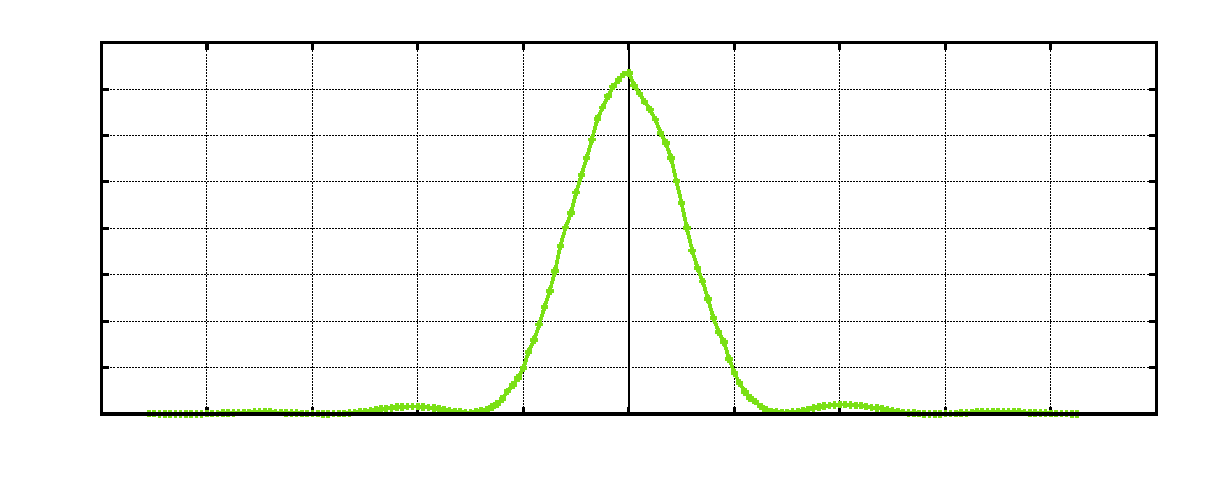
\includegraphics{jedna_szczelina}}%
    \gplfronttext
  \end{picture}%
\endgroup
}		
			\caption{W zwykłej skali.}
			\label{jedna_szczelina}
        \end{subfigure}%
        ~ %add desired spacing between images, e. g. ~, \quad, \qquad, \hfill etc.
          %(or a blank line to force the subfigure onto a new line)
          
        \begin{subfigure}[b]{\textwidth}
			\fontsize{6}{8}\selectfont % zmniejszam czcionke
			\centering
			\resizebox{0.9\textwidth}{!}{% GNUPLOT: LaTeX picture with Postscript
\begingroup
  \makeatletter
  \providecommand\color[2][]{%
    \GenericError{(gnuplot) \space\space\space\@spaces}{%
      Package color not loaded in conjunction with
      terminal option `colourtext'%
    }{See the gnuplot documentation for explanation.%
    }{Either use 'blacktext' in gnuplot or load the package
      color.sty in LaTeX.}%
    \renewcommand\color[2][]{}%
  }%
  \providecommand\includegraphics[2][]{%
    \GenericError{(gnuplot) \space\space\space\@spaces}{%
      Package graphicx or graphics not loaded%
    }{See the gnuplot documentation for explanation.%
    }{The gnuplot epslatex terminal needs graphicx.sty or graphics.sty.}%
    \renewcommand\includegraphics[2][]{}%
  }%
  \providecommand\rotatebox[2]{#2}%
  \@ifundefined{ifGPcolor}{%
    \newif\ifGPcolor
    \GPcolortrue
  }{}%
  \@ifundefined{ifGPblacktext}{%
    \newif\ifGPblacktext
    \GPblacktextfalse
  }{}%
  % define a \g@addto@macro without @ in the name:
  \let\gplgaddtomacro\g@addto@macro
  % define empty templates for all commands taking text:
  \gdef\gplbacktext{}%
  \gdef\gplfronttext{}%
  \makeatother
  \ifGPblacktext
    % no textcolor at all
    \def\colorrgb#1{}%
    \def\colorgray#1{}%
  \else
    % gray or color?
    \ifGPcolor
      \def\colorrgb#1{\color[rgb]{#1}}%
      \def\colorgray#1{\color[gray]{#1}}%
      \expandafter\def\csname LTw\endcsname{\color{white}}%
      \expandafter\def\csname LTb\endcsname{\color{black}}%
      \expandafter\def\csname LTa\endcsname{\color{black}}%
      \expandafter\def\csname LT0\endcsname{\color[rgb]{1,0,0}}%
      \expandafter\def\csname LT1\endcsname{\color[rgb]{0,1,0}}%
      \expandafter\def\csname LT2\endcsname{\color[rgb]{0,0,1}}%
      \expandafter\def\csname LT3\endcsname{\color[rgb]{1,0,1}}%
      \expandafter\def\csname LT4\endcsname{\color[rgb]{0,1,1}}%
      \expandafter\def\csname LT5\endcsname{\color[rgb]{1,1,0}}%
      \expandafter\def\csname LT6\endcsname{\color[rgb]{0,0,0}}%
      \expandafter\def\csname LT7\endcsname{\color[rgb]{1,0.3,0}}%
      \expandafter\def\csname LT8\endcsname{\color[rgb]{0.5,0.5,0.5}}%
    \else
      % gray
      \def\colorrgb#1{\color{black}}%
      \def\colorgray#1{\color[gray]{#1}}%
      \expandafter\def\csname LTw\endcsname{\color{white}}%
      \expandafter\def\csname LTb\endcsname{\color{black}}%
      \expandafter\def\csname LTa\endcsname{\color{black}}%
      \expandafter\def\csname LT0\endcsname{\color{black}}%
      \expandafter\def\csname LT1\endcsname{\color{black}}%
      \expandafter\def\csname LT2\endcsname{\color{black}}%
      \expandafter\def\csname LT3\endcsname{\color{black}}%
      \expandafter\def\csname LT4\endcsname{\color{black}}%
      \expandafter\def\csname LT5\endcsname{\color{black}}%
      \expandafter\def\csname LT6\endcsname{\color{black}}%
      \expandafter\def\csname LT7\endcsname{\color{black}}%
      \expandafter\def\csname LT8\endcsname{\color{black}}%
    \fi
  \fi
  \setlength{\unitlength}{0.0500bp}%
  \begin{picture}(11338.00,4534.00)%
    \gplgaddtomacro\gplbacktext{%
      \csname LTb\endcsname%
      \put(946,704){\makebox(0,0)[r]{\strut{}$0.01$}}%
      \csname LTb\endcsname%
      \put(946,1595){\makebox(0,0)[r]{\strut{}$0.1$}}%
      \csname LTb\endcsname%
      \put(946,2487){\makebox(0,0)[r]{\strut{}$1$}}%
      \csname LTb\endcsname%
      \put(946,3378){\makebox(0,0)[r]{\strut{}$10$}}%
      \csname LTb\endcsname%
      \put(946,4269){\makebox(0,0)[r]{\strut{}$100$}}%
      \csname LTb\endcsname%
      \put(1078,484){\makebox(0,0){\strut{}$-10$}}%
      \csname LTb\endcsname%
      \put(2064,484){\makebox(0,0){\strut{}$-8$}}%
      \csname LTb\endcsname%
      \put(3051,484){\makebox(0,0){\strut{}$-6$}}%
      \csname LTb\endcsname%
      \put(4037,484){\makebox(0,0){\strut{}$-4$}}%
      \csname LTb\endcsname%
      \put(5023,484){\makebox(0,0){\strut{}$-2$}}%
      \csname LTb\endcsname%
      \put(6010,484){\makebox(0,0){\strut{}$0$}}%
      \csname LTb\endcsname%
      \put(6996,484){\makebox(0,0){\strut{}$2$}}%
      \csname LTb\endcsname%
      \put(7982,484){\makebox(0,0){\strut{}$4$}}%
      \csname LTb\endcsname%
      \put(8968,484){\makebox(0,0){\strut{}$6$}}%
      \csname LTb\endcsname%
      \put(9955,484){\makebox(0,0){\strut{}$8$}}%
      \csname LTb\endcsname%
      \put(10941,484){\makebox(0,0){\strut{}$10$}}%
      \put(176,2486){\rotatebox{-270}{\makebox(0,0){\strut{}Natężenie Światła $I$}}}%
      \put(6009,154){\makebox(0,0){\strut{}Odległość $x$ [mm]}}%
    }%
    \gplgaddtomacro\gplfronttext{%
    }%
    \gplbacktext
    \put(0,0){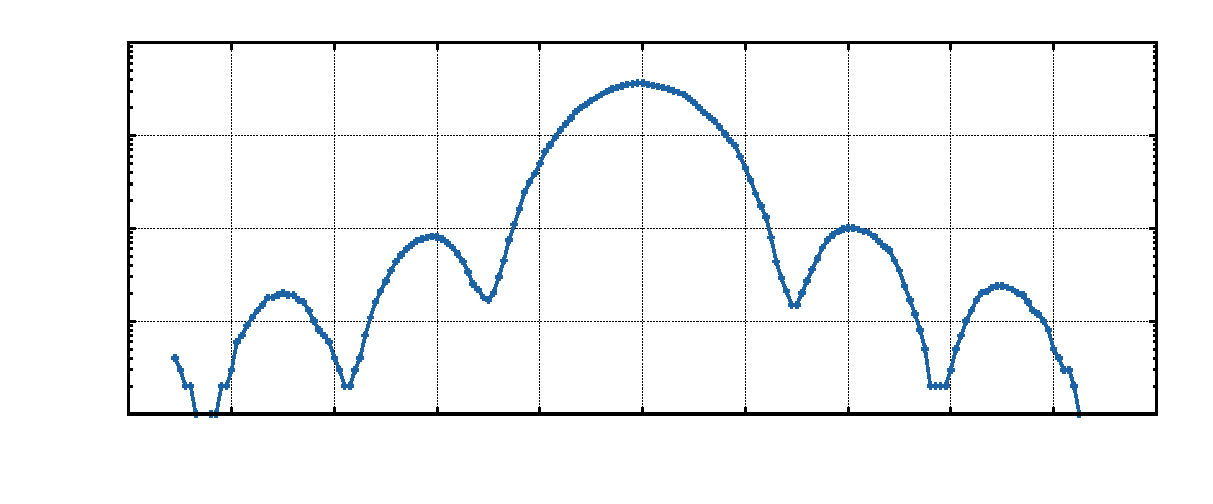
\includegraphics{jedna_szczelina_log}}%
    \gplfronttext
  \end{picture}%
\endgroup
}	
			\caption{W skali półlogarytmicznej}
			\label{jedna_szczelina_log}
        \end{subfigure}
        ~ %add desired spacing between images, e. g. ~, \quad, \qquad, \hfill etc.
          %(or a blank line to force the subfigure onto a new line)
        \caption{Wykres zależności natężenie światła $I$ od położenia detektora $x$.}\label{jedna_szczelina_calosc}
\end{figure}

\begin{table}[h!]
\centering
\caption{Położenia maksimów i minimów natężenia światła}
	\begin{tabular}{|C{2cm}|C{2cm}|C{2cm}|C{2cm}|C{2cm}|}\hline
		Element obrazu dyfrakcyjnego & Położenie z lewej $x_l$ [mm] & Położenie z prawej $x_p$ [mm] & $x = \frac{x_p-x_l}{2}$ [mm] & Obliczona szerokość szczeliny $d$ [mm] \\ \hline
		1 minimum & -3,0 & 2,9 & 2,95 & $0,02375$\\ \hline
		1 maksimum boczne & -4,1 & 4,1 & 4,1 & $0,02563$ \\ \hline
		2 minimum & -5,8 & 5,6 & 5,7 &  $0,02458$ \\ \hline
		2 maksimum boczne & -7,0 & 6,9 & 6,95 & $0,02520$\\ \hline
	\end{tabular}
\label{jedna_szczelina_tab_maks}
\end{table}



\newpage
%%%%%%%%%%%% BIBLIOGRAFIA %%%%%%%%%%%%
\begin{thebibliography}{9}
	
	\bibitem[1]{1}
	Z. Stęgowski,
	\emph{Zeszyt A1 do ćwiczeń laboratoryjnych z fizyki}, Kraków, Akademia Górniczo Hutnicza im. Stanisława Staszica, dostępny na stronie:\\
	\url{http://www.fis.agh.edu.pl/\~pracownia\_fizyczna/cwiczenia/71\_opis.pdf}
	
	
	
	\bibitem[2]{}
	Jacek Tarasiuk,
	\emph{Wykłady, Statystyka Inżynierska} , Kraków, Akademia Górniczo Hutnicza im. Stanisława Staszica, dostępny na stronie:\\
	\url{http://home.agh.edu.pl/~tarasiuk/dydaktyka/index.php/statystykainzynierska}
	
	\bibitem[3]{3}
	Andrzej Zięba,
	\emph{Opracowanie danych pomiarowych}, Kraków, Akademia Górniczo Hutnicza im. Stanisława Staszica, dostępny na stronie:\\
	\url{http://www.ftj.agh.edu.pl/zdf/danepom.pdf}
	\label{statystyka}
	
	\bibitem[4]{4}
	Andrzej Zięba,
	\emph{Pracownia fizyczna wydziału Fizyki i techniki jądrowej AGH} , wydawnictwa AGH, Kraków, 1999\\
	
	
	\bibitem[5]{5}
	D.Halliday, R.Resnick
	\emph{Fizyka dla studentów nauk przyrodniczych i technicznych.} Tom II, wydanie III, PWN, Warszawa 1974
	
\end{thebibliography}





\end{document}



